\documentclass[11pt]{article}
\usepackage[a4paper,pdftex]{geometry}
\setlength{\oddsidemargin}{5mm}
\setlength{\evensidemargin}{5mm}
\usepackage[english]{babel}
\usepackage{amsmath,amsfonts,amsthm,amssymb}
\usepackage{graphicx}
\usepackage{fancyhdr}
\pagestyle{fancy}
\usepackage{url}
\usepackage{lastpage}
\urlstyle{same}

% Page numbering
\lhead{SmartClass: Optimizing Education}
\rhead{page \thepage/\pageref{LastPage}}
\cfoot{}
\rfoot{\thepage}

% TITLE FORMAT
\newcommand{\HRule}[1]{\rule{\linewidth}{#1}}

\makeatletter
\def\printtitle{
    {\centering \@title\par}}
\makeatother                  

\makeatletter
\def\printauthor{
    {\centering \large \@author}}
\makeatother

% TITLE
\title{
\HRule{0.5pt} \\
\LARGE \textbf{\textsc{SmartClass}}\\[0.5cm]
\normalsize \textsc{Optimizing Education}
\HRule{2pt}\\ [0.5cm]
\normalsize
\today
}

\author{
\vspace{1.5cm}
Supervised by dr. F. Nack and M. S. Latour\\[0.5cm]
\begin{tabular}{c c c c}
M. A. Cabot & S. Laan & C. R. Verschoor & A. J. Wiggers\\
6047262 & 6036031 & 10017321 & 6036163
\end{tabular}\\[0.5cm]
Artificial Intelligence\\
Faculty of Science\\
Universiteit van Amsterdam\\
}

% BEGIN DOCUMENT
\begin{document}

% TITLE PAGE
\thispagestyle{empty}
\printtitle                  
\vfill
\begin{abstract}
\noindent This paper describes a design of a knowledge media application for universities based on the user experience of lectures in university. The application, called SmartClass, gathers data from the user, internet and previous presentations in order to create new presentation slides based on the feedback of users. The application focuses on the individual experience of the users: the teacher and the student. All processed data is represented in OWL/RDF format, to provide a reasoning logic that can run queries in our ontology and browse through the available data. The user can ask questions about specific elements of the presentation. The application searches the information about this query and presents this to the user on newly generated slides. The application contains a self learning system that improves the presentation based on feedback, namely the approval or denial of slides and the amount of questions asked.
\end{abstract}
\printauthor
\newpage

% TABLEOFCONTENTS
\setcounter{page}{1}
\tableofcontents
\newpage

% CONTENT
\section{Introduction}
This paper shows the framework of a knowledge based multimedia system designed to generate new slides for a presentation in two scenarios. The first scenario is when the system generates new slides for the lecturer offline, improving on the slides that were used the year before. The second scenario is when the system generates a personal slide, online, for a student who has a question about the given lecture. In this case offline means that generation of presentation slides happens before the presentation and online means that the application generates real time the presentation slides

In the next sections the following aspects regarding the application are described: the user groups, the design and concepts, the application from student perspective, the application from teacher perspective, the interface of the applications and lastly the application is discussed. 

\section{User groups}
The system is designed with a specific group of users in mind. There are two main user groups, which will be described in this section.

\subsection{Teacher}
The first group of users is the group of teachers. This group has the most control over the system. It is important that the system gives teachers this control without distracting them from their main task, i.e. giving a lecture.

\subsection{Students}
The other user group is the group of students. Students will only use the system during lectures. We distinguish between three stereotypical `students’:
\begin{itemize}
\item The Normal Student pays attention during lectures. When he has a question it will be an in-depth question. He wants to know more than is necessary.
\item The Lazy Student is lazy. The student does not take notes, does not pay attention, or at least not the whole time. In general, the student will not ask any questions. The only exception is when a subject is discussed that appeals to him/her personally. He/she might also ask sarcastic questions.
\item The Not That Smart Student is a bit slower of understanding. He/she is always a few steps behind. Whenever he/she asks a question, it might have already been answered, the student just did not notice the answer. Other questions from this student include questions about concepts that are considered known, but he/she forgot.
\end{itemize}

\section{Application Design and Concepts}
The application will allow users to access the newly generated content in two ways: Firstly, by generating new presentations based on previous presentations. Secondly, by generating a new presentation slide based on the question asked by the user. This section describes the concepts that are used to design the SmartClass application.
% Note above sentence has to be better. 
% Is this better?

\subsection{Information Gathering}
The application gathers information from the following sources:
\begin{description}
\item[Student user of the application.] The amount of questions users ask concerning a presentation slide indicates the value of the slide (feedback to the application).
\item[Teacher user of the application.] Whether a teacher presents or deletes a newly generated presentation slide (feedback to the application).
\item[Encyclopedia or content related websites.] To automatically generate a new presentation slide containing the answer to the question.
\item[Previous generated slides.] To generate new presentation slides based on the performance of previous presentation slides.
\end{description}

\subsection{Displayed information}
The application displays various information for both the user groups. This section describes the displayed information for both student and teacher. How the information changes based on the systems input is described in the next section. 
\subsubsection{Student}
The application displays the following information to the users that are students:
\begin{description}
\item[Presentation slides.] The generated slides of the teacher are displayed, so the student can follow the presentation given by the teacher. The student has the option to browse through the presentation slides or to automatically follow the teacher's presentation slides.
\item[Asked questions.] Questions asked by students will be displayed in the Quick Question Box, which is described in a later section. % Reference should be added 
\item[Automatically generated presentation slides.] The system generates answer slides according to the question asked by the students.
\item[Notes.] The student can freely scroll through the notes that accompany each slide and add information to notes of previous or upcoming slides as well. The student has the ability to draw and/or write these notes.
\end{description}

\subsubsection{Teacher}
The application displays the following information to the users that are teacher:
\begin{description}
\item[Presentation slides.] The generated slides are displayed, so the teacher sees the generated presentation in front. The teacher can comfortably view and present the presentation slides.
\item[Asked questions.] The top and unanswered questions are displayed, so the teacher sees the questions of the student, while giving its presentation. It's up to the teacher to decide if en when to discuss a question using a generated slide. 
\item[Automatically generated presentation slides.] The system generates answer slides according to the question asked by the students. The teacher has the ability to reject or use the generated presentation slide.
\item[Notes.] The teacher has the ability to use speaker notes while giving the presentation in order to prepare the presentation.
\end{description}

\subsection{User Contribution}
There are various ways to influence the output of the system. This section will describe the influence of every user of the application.
\subsubsection{Student}
Every user that is a student has three options:
\begin{description}
\item[Asking questions.] A visual change in output is that the question will appear in the question box. The system will also try to find additional information about the subject that might help answer the question.
\item[Voting in favor or in disfavor of questions.] A voting system is used to determine the importance of unanswered questions. Users can vote for a question if they also want additional information about the subject. The questions with the most votes appear at the top of the question box to indicate that these have the highest priority.
\item[Making notes.] As these notes are personal, they will not change the output for other users. When the user is taking notes of a certain presentation slide, the student can go back to the concerning presentation slide.
\end{description}

\subsubsection{Teacher}
Users that are teachers have these options: 
\begin{description}
\item[Deleting generated slides.] A teacher has to approve of each slide before they are used in the presentation. This is to avoid confusion and to leave out irrelevant and unnecessary information.
\item[Using generated slides.] When a teacher decides that he/she will use the generated slide, it is incorporated in the presentation. 
\end{description}

\subsection{Information Searching}
A search for information is necessary if new slides are to be generated.
\begin{itemize}
\item When a question is asked, there are two important features for this question.
\begin{itemize}
\item The domain of the question. This is determined by the slide at which it was asked. 
\item Textual input. Keywords in the question (e.g. `where’, `when’, `how’) and the use of concepts (e.g. cockpit in a presentation about airplanes) are the most important.
\end{itemize}
\item When a new presentation is generation the application uses two important features of the slide to finds new content related to the slide.
\begin{itemize}
\item Domain of the slide. This is determined by the previous presentation and its feedback
\item Meta-information. Slide representation contains extra information about the slide.
\end{itemize}
\end{itemize}

\subsection{Self learning system}
The system will use machine learning methods to improve itself. There are multiple features that can tell the system how well it is functioning:
\begin{description}
\item[Student questions.] Several questions for one slide indicate that this slide is not very clear or that the slide needs additional information.
\item[Approval by teachers.] Since the teacher can approve or reject newly formed slides, the system can learn which slides are favorable. Of course, this does lead to a biased idea of a good slide, since the teacher may have a wrong idea about slide creation.
\item[Test results.] When several students make mistakes concerning one particular subject, it needs extra coverage. The system should be able to provide additional slides about this particular subject.
\end{description}

\subsection{Slide Representation}
Each slide (or combination of slides) should contain the following components:
\begin{description}
\item[The title.] It addresses the main topic of the current slide.
\item[Bullet points.] Each bullet point is related/linked to the title.
\item[Text.] Each piece of text is related/linked to a bullet point.
\item[Images.] Each image is related/linked to a bullet point.
\end{description}

\subsection{Offline generation}
Offline generation is the act of generating new slides for the presentation based on the previous slides. This action is performed before a lecture so that the teacher knows what the slides will look like. Depending on the representation of the previous presentation one of two types of offline generation is performed. The first time a lecture is given using this system the previous slides do not have the required representation. In this case the system must place the content of the old slides in the representation used by the system. If the previous slides already have the required representation, then the new presentation can be improved by adding slides that answered popular questions. The teacher is able to reject, alter or add new slides.

\subsection{Online generation}
A student is able to ask a question about every element of a slide by clicking on it. Online generation is the act of generating a new slide in real-time that answers the student's question. We distinguish between two types of questions: definition- and open-questions.

A definition-question is a question about the definition of a term. The system create a slide that has as title the selected term and as content the definition of that term. If available, an image can be added to clarify the definition. This type op question will be especially helpful for the forgetful and less intelligent student. 

An open-question is any question other than a definition-question. Of all the information available about the term in question, only the information that is relevant to the question needs to be displayed on the new slide. The relevant information is selected by decomposing the question into a subject, relation and object. One of these parts is the selected term (what the question is about) and another is the thing that needs to be answered. What essentially needs to happen is that the question is translated into a RDF query. A RDF query can then be used to find the relevant information on the internet. After retrieving the relevant information a slide can be generated according to the slide representation explained above.

\subsection{Quick Question Box}
The Quick Question Box (QQB) is displayed on both the students’ interface as well on the teacher's interface. The QQB contains a list of questions that have been asked by the students. Each question is linked to its generated slide (only if an answer could be generated). This gives students, especially lazy students, easy access to extra information without having to type the question themselves. As stated before, each question can be voted up or down and are sorted by their number of votes. This gives the teacher an overview of the questions that are puzzling most students. The teacher can then choose to cover a question with the whole class using the slide generated to answer this question. The teacher has also the option to deny a slide, when it is not covering the question at all in order to give feedback to the system.

\subsection{Notes}
As stated before, beneath every slide a student is able to make his/her notes. After a lecture the student will be able to extract a file containing the slides with his notes. 

\section{Student Perspective}
SmartClass was designed with the following in mind: `What would the student expect from a system that enhances lectures?’. The system should be able to make a lecture a more complete and more interesting learning experience than a regular lecture. Not only does it encourage students to actively participate and ask questions, it also enables them to give feedback on the slides and presentation indirectly. 
The questions can be asked anonymously. This makes the asking of questions even more easy accessible. A few problems arise when it comes to asking questions during a lecture:
\begin{itemize}
\item Students may fear interrupting the teacher.
\item Students may think that their question is not a very good one.
\item Students may think that their question involves something that has already been answered earlier in the lecture.
\item And if we reverse this problem: A teacher may be interrupted by questions that involve earlier parts in the slides (if the student was not paying attention).
\end{itemize}
All these problems are solved by SmartClass:\\
Asking a question via the Quick Question Box does not immediately interrupt the teacher. If the question can be answered by the system alone using new or previous slides, then the problem is solved. If this is not the case and it is a good, relevant question then other students may vote in favor of it. It will then reach the top of the box where it is clearly visible for the teacher, who can then choose to either use the slide that attempted to answer the problem and explain it further or just explain the answer without using these slides. Since students are free to scroll through the slides themselves, they will be able to see if their question has not already been answered, thus leaving more time for relevant and new questions.

\section{Teacher Perspective}
Many teachers use the slides of previous years as a guideline for the next year, or sometimes even copy them entirely. In the first case, it will cost a significant amount of time to adjust the slides manually. In the second case, the slides may be outdated, new techniques or discoveries might have been made that require the slides to be adjusted. In both cases, SmartClass comes in handy.  Generation of new slides happens based on slides of previous years but the system looks at new sources simultaneously. These slides can still be fully edited giving the teacher full control over the content of his/her presentation.

The presentation panel and speaker notes of the teacher interface are designed to be intuitive and similar to the way `normal’ presentations are given. In addition, the teacher now has the QQB allowing him/her to be aware of pressing questions by students. Again, the teacher is in control of the content being shown. SmartClass leaves it up to the teacher to decide whether a newly generated slide is to be displayed. 

\section{User Interface}
In this section the interface is discussed of the interface.
\begin{figure}[!h]
\centering
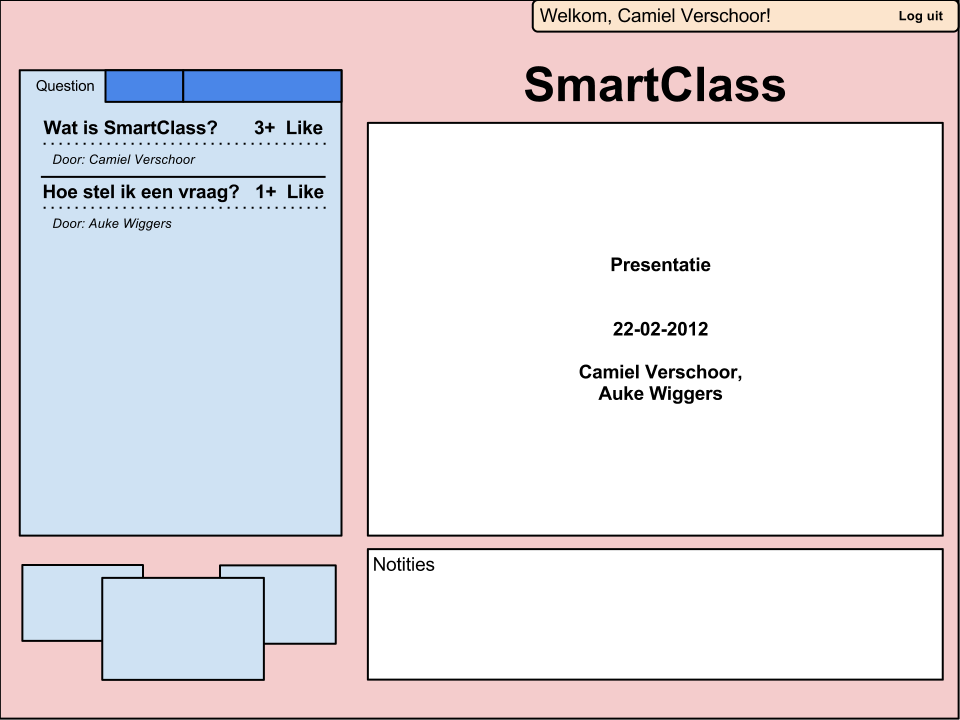
\includegraphics[width=0.7\textwidth]{KBMSInterface.png}
\caption{A schematic of the interface, questions are not anonymous here}
\end{figure}
\subsection{Student}
\subsubsection{Main Window}
The main window is where the most time is spent. It consists of the following components shown in the above figure.
\begin{description}
\item[1. Quick Question Box] In the Quick Question Box the best questions are shown together with the number of votes. The questions can be clicked. On clicking the generated slide for that question is shown. Each question is accompanied by two buttons that allow a user to vote in favor or in disfavor of the question. 

\item[2. The Presentation Panel] In the presentation panel slides are shown. The keywords on the slides can be clicked. On clicking the Question Dialog will popup. By default, the slide on the presentation panel automatically synchronizes with the slide being discussed by the teacher. An exception is when a student is making notes about a slide. In this case the panel will synchronize after the student is done making notes. It is also possible to toggle the synchronization off or on manually.  

\item[3. Navigation Thumbnails] The navigation thumbnails are little previews of the slides to come and the slides that already have been showed. They can be used to navigate through the presentation.

\item[4. Notes Textbox] In the Notes Textbox, the student can make notes. These notes will be linked to the slide that is currently shown (in the presentation panel, which is not essentially the same as the slide the teacher is showing). The textbox is scrollable. When moving from one note to another, the slides will move accordingly. 
\end{description}

\subsubsection{Question Dialog}
The question dialog is a popup window in which the student can type a question or hit the definition-button.

\subsection{Teacher}
\subsubsection{Main Window}
\begin{description}
\item[1. Quick Question Box] By default, the question box looks the same as that of the students. The difference is that when a teacher clicks a question, it will lead him to a preview of the slide which he/she can then choose to incorporate in his/her presentation by clicking the `accept’ button. 

\item[2. The Presentation Panel] Just as in the students interface, the presentation panel shows the current slides. Since the teacher is the one in charge of scrolling through the slides, there is no option for synchronization. 

\item[3. Preview box] In this box, the teacher will be able to see a pre-generated slide after clicking a question. The teacher is able to include one of these slides in his/her presentation. 

\item[4. Notes Textbox] In the Notes Textbox, the teacher can see personal notes that he/she made beforehand. It is usually easier to give a presentation if some keywords are written down beforehand, synchronizing them with the slides only makes it easier. The teacher does not have the ability to make new notes during the presentation, only beforehand.
\end{description}
\subsection{Student and Teacher}
\subsubsection{Login System}
The application uses the Central Authentication Service (CAS) of the University of Amsterdam to allow users to access the application. This enables the system to save the users personal data (such as notes or question) without having to register on our application. CAS allows web applications to authenticate users without gaining their security credentials. Since every user of the application has an account at the university, this service fits in our application. In the figure below a picture of the CAS login screen.
\begin{figure}[!h]
\centering
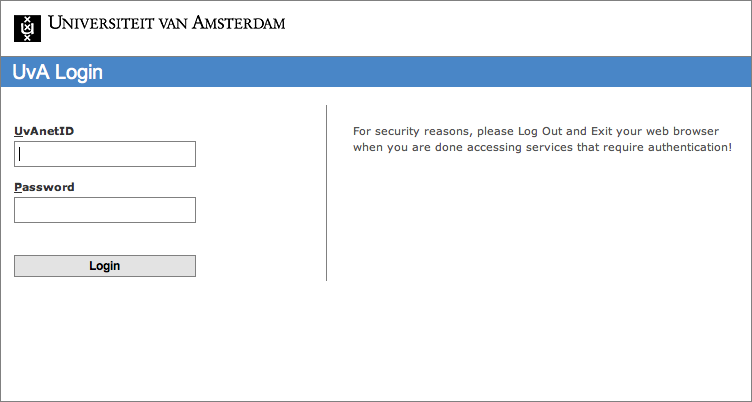
\includegraphics[width=0.7\textwidth]{Cas.png}
\caption{Central Authentication Service login screen}
\end{figure}
\section{Discussion}
Under construction
\end{document}
​